\documentclass[letter, 10pt, conference]{ieeeconf}
\usepackage{graphicx}
\usepackage{cite}

\setlength{\parskip}{1em}
% \renewcommand{\baselinestretch}{1.1}

\title{\LARGE \bf A distributed real-time simulation based approach for quantifying CO$_2$ emissions of urban car traffic}

\author{ \parbox{4 in}{ \centering Juan Carlos Ramos Martínez \\
  Institute of Computer Science\\
  University of Tartu}}

\begin{document}

\maketitle
\thispagestyle{empty}
\pagestyle{empty}

%%%%%%%%%%%%%%%%%%%%%%%%%%%%%%%%%%%%%%%%%%%%%%%%%%%%%%%%%%%%%%%%%%%%%%%%%%%%%%%%

\begin{abstract}

Traffic CO$_2$ emission is a constant problem that have an impact into the environment.
There are proposed solutions that improve the traffic analysis and operation performance to reduce traffic congestion and increase overall safety.
However, these solutions have become increasingly complex due to the inclusion of multiple tools for treating the traffic management at a realistic manner.
Emission models, that represent a separate complex task on its own, have been introduced in these systems making them even more difficult to scale.
ITS needs to have easy and effective mechanisms for interacting with the existing vehicle infrastructure and be able to accomplish one task right.
This paper explores the implementation of a system that focuses on the gathering and calculation of CO$_2$ emissions of urban vehicle traffic.
The system presented is a cloud-based infrastructure that has been tested using different simulation scenarios with the objective of provide realistic urban traffic behaviour.
The paper also looks at the value of having a wide range of perspectives to evaluate transport pollution based on the existing retrieved information.

\end{abstract}

%%%%%%%%%%%%%%%%%%%%%%%%%%%%%%%%%%%%%%%%%%%%%%%%%%%%%%%%%%%%%%%%%%%%%%%%%%%%%%%%
\section{INTRODUCTION}

In most urban areas traffic congestion has become a regular problem.
Traffic is responsible for a significant portion of urban energy consumption (releasing emissions such as CO$_2$, CH$_4$, N$_2$O, and others) \cite{patterson_preparing_nodate}.
This comes with a impact in the environment \cite{karagiannis_vehicular_2011}.
For such extent, scientific and industrial communities are working on issues related to congestion of vehicle traffic, mainly Intelligent Transport Systems (ITS).
Recently, there has been interest for integrating such solutions with a wide variety of emission models.
They differ in the required input parameters, the aggregation of results, and the coverage of real-world population of vehicles \cite{hofer_large_2018}.
Emissions are affected by the way the vehicle is driven, taking into consideration parameters such as speed, acceleration, vehicle slope between the most important ones \cite{noauthor_intergovernmental_2001}.
Academic methods, such as the Simulation of Urban Mobility (SUMO) or Multi Agent Transport Simulation (MatSIM), aim to simulate at microscopic level traffic and emission behavior \cite{bazzan_multi-agent_2009}.
Moreover, these are the most widely used simulation tools that enable realistic traffic environments.
Specifically, the SUMO simulator is more convenient due to the exposure of the TraCI protocol that is used for collecting data of individual vehicle on runtime (i.e. speed, position, acceleration, etc).
However, these methods use independent methods to approach the single task of CO$_2$ emission.

On the other hand, Internet of Things (IoT) has appeared as a solution for a data-driven model that allow people, businesses, and service providers interact with the environment.
Cloud computing has become cost-effective and popular technology for efficient use of distributed resources.
It allows to process large volumes of data and solve large-scale problems.
This is precisely what IoT needs to scale and operate well on a real world scenario.
Many IoT architectures have tried to integrate the vehicle network with cloud data processing with promising results \cite{tarneberg_experiences_2016}.
However, there are not many efforts which use a IoT network for the assessment of calculating the CO$_2$ emissions of a network of vehicles.

In any case, traffic models are usually the starting point for calculate the amount of pollutants emitted.
One way to test a IoT system that focuses on specific tasks is through the usage of appropriate traffic simulators at microscopic level.
This paper focuses on the structure and implementation of a system that is capable of calculate the emission of CO$_2$ on vehicle network in real-time.
More specifically, the presented approach uses a simulator to send telemetry data to a IoT Gateway, via TraCI protocol, to a connected vehicle ecosystem.
This is essential for the scalability and reliability of the connected devices with specific parameters in real world scenarios.

The following section provides an overview of the existing IoT and Emission simulation approaches.
Section 3 introduce the process of implementing the system, addressing the integration of the protocol TraCI for simulation, and usage of useful tools for visualization.
A cloud-based example of vehicle traffic is introduced in the Section 4. This will be used as a basis for evaluating the usability of the system.
Finally, Section 5 presents the conclusions and future work.

%%%%%%%%%%%%%%%%%%%%%%%%%%%%%%%%%%%%%%%%%%%%%%%%%%%%%%%%%%%%%%%%%%%%%%%%%%%%%%%%
\section{RELATED WORK}

This section provides a brief overview of related approaches to simulate and build systems on the traffic domain found in the literature.

\subsection{ITS Systems and IoT}

Some ITS systems have been created to provide better traffic management \cite{de_souza_real-time_2016} \cite{brennand_intelligent_2015}.
Such systems rely on the identification and recommendation of alternative routes for vehicles based on the information they provide on a regular basis.
However, ITS systems that use centralized approach tend to overload the network when the flow of vehicle is increased \cite{de_souza_fully-distributed_2016}.
Decentralized approaches suffer the same problem when they incur into vehicle communication \cite{de_souza_fully-distributed_2017}.

These approaches usually rely on well-know traffic simulators that helps in the understanding and explaining process.
For example, traffic behavior can be related to the actual system being studied.
In this context, there have been intents for using the power of Internet-of-Things (IoT) into simulators.
Previous work \cite{waddell_architecture_2018} presented an extensive analysis of existing simulators taking into consideration: big data processing, network simulation and architecture domain.
Nonetheless, none of the simulators considered were specifically designed to microscopically simulate traffic scenarios relying on vehicle-specific data.
More recently \cite{hofer_large_2018} presented an approach that uses SUMO simulator in conjunction with Eclipse Kuksa to bring microscopic simulation that supports networks, traffic transport and pedestrians.
They even presented an emission calculation of traffic into their simulations.
However, they focus on the integration with the proprietary cloud platform Kuksa, which contains features that are beyond the simulation domain.
Moreover they present limitations regarding to real-time support, and highlights the drawback of using SUMO for testing and tunning specific complex scenarios.
Previous effort for bringing a cloud-based infrastructure to support systems that simulate real-work environments of traffic networks within the IoT domain has been discussed in \cite{tarneberg_experiences_2016}.

\subsection{Traffic and emission simulation}

There are many different ways of simulating traffic and there are particular benefits and drawbacks for all strategies.
Most traffic models are designed from the bottom up, i.e. starting from single-vehicle activity and aggregating to produce macro-scale performance.

The most famous model is based on Cellular Automata proposed by Nagel-Schreckenberg \cite{nagel_cellular_1992}.
There are also agent-based models which includes pedestrian movement and more complex behaviors.
In addition, driving patterns such as speed and acceleration are crucial in estimating emissions and fuel consumption of vehicles \cite{markiewicz_reduction_2017}.

For a complete reference of traffic simulations refer to \cite{kotusevski_review_nodate}.
A variety of open source and commercial simulation tools are available due to ongoing research and development, they are primarily based on these rule-based mechanics.
SUMO is generally better suited for multi-modal simulations (macroscopic, microscopic and mesoscopic).
Microscopic simulation on SUMO have the advantage of producing a wide variety of emission pollutant outputs which may be useful for having a broad overview of specific scenarios.

Even though there are currently advanced methods for simulate urban and traffic emissions, a new method for bringing the emission calculation into the system is needed.

The main advantages for the proposed approach is:
\begin{itemize}
\item to accommodate into the current vehicle network
\item to visualize and have tools for filtering data
\item to run on a real-world map
\item to adapt into possible developments and pollutant types
\end{itemize}

%%%%%%%%%%%%%%%%%%%%%%%%%%%%%%%%%%%%%%%%%%%%%%%%%%%%%%%%%%%%%%%%%%%%%%%%%%%%%%%%
\section{PROPOSED SOLUTION}

The purpose of this system is to calculate the emissions caused by a connected urban car traffic in real-time.
This is archived in multiple steps.
The paper begins by addressing the approach by defining the components and system properties.
Then, the design of the system architecture is presented in section B, followed by the a web application that serves as a visualization tool.
In the remainder of this section, the road network is generated and detailed.
Then the simulation and implementation of CO$_2$ emission per vehicle is developed.
For this, SUMO simulator is used in a predefined and stable network.
The generation of CO$_2$ emissions is compared to a ground truth made by SUMO emission output.
The possibilities of the system is discussed at the end.

\begin{figure}[h]
  \centering
  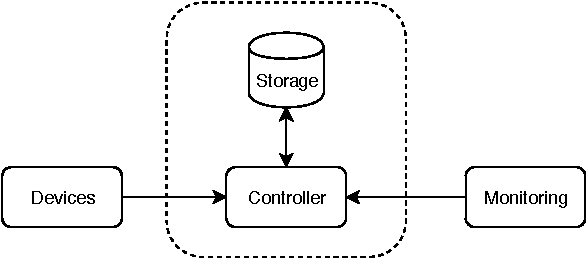
\includegraphics[width=0.45\textwidth]{diagram1}
  \caption{Components of the system}
  \label{fig:diagram1}
\end{figure}

\subsection{System Components}

The presented system relies on connected devices representing the vehicles.
The paper focuses on gathering the data and calculating CO$_2$ emission based on it.
For this we need to define the components that are needed to construct the system (see Figure \ref{fig:diagram1})

\subsubsection{Devices}

The system will collect data from a set of connected devices.
These devices may not be able to report successfully at the desired rate due to intermittent connectivity.
Additionally, this reported data contains a certain rate of error.

\subsubsection{Storage}

Storage Data collected by devices store the current state of the device entities.
They are processed before being stored.
The data is also stored for current and future analysis.

\subsubsection{Controller}

The system operates with a controller that acts on the input from devices in real-time.
Then the data is stored and preprocessed into the storage component.
The controller is also used to retrieve data for the Web client application.

\subsubsection{Monitoring}

The processed data is displayed in a web component that contains tools for visualization.
This operates by collecting up and grouping the data of the storage component.

\subsection{System Implementation}

Having the picture of the system components in mind, the task now is to implement it in a way that allows connectivity among the vehicles to later process their individual data.
As shown in Figure \ref{fig:diagram2}, the entry point to the cloud platform is a message gateway that links vehicles and other devices in a flexible and integrated way to cloud services.
For doing so, the gateway accepts, sends, and receives messages from and to the vehicles.

The back-end application acts as the message gateway by providing communication over HTTP and potentially over the MQTT protocol.
Then, a time-series database, namely InfluxDB, is used to storage received messages as a real time telemetry of vehicles.
Data from traffic is published to a common data channel into a stream end-point.
Vehicles emit messages to the controller containing the entity id, speed, latitude, longitude, and acceleration.
The messages are processed by a function that calculates the emission based on these attributes.
It is then possible for the emission to be calculated concurrently.
This ensures multiple evaluations while ensuring processing in real time.
The result, along with the vehicle information is stored in a database table defined in Figure \ref{fig:db_schema}.

\begin{figure}[h]
  \centering
  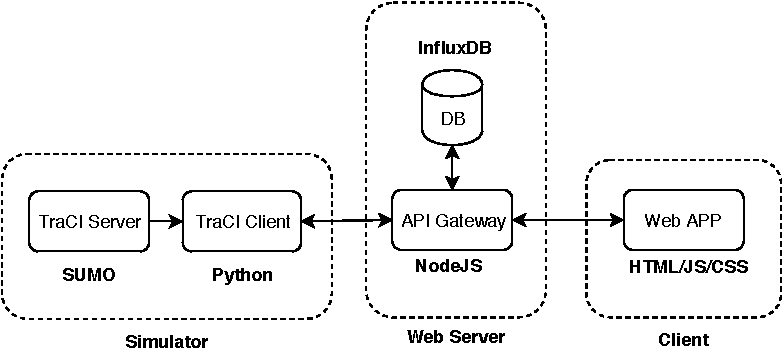
\includegraphics[width=0.45\textwidth]{diagram2}
  \caption{System components of the simulated implementation}
  \label{fig:diagram2}
\end{figure}

At this point, the system contains the data accumulated in the database in a way that is easy to be retrieved.
NodeJS will perform any interactions with the database using the appropriate controller \footnote{https://github.com/influxdata/influxdb-python} for the task.
It is then possible for other services to fetch the information from the database for further processing and visualization.
One example for such service is a web application which visualizes the vehicle related information CO$_2$ emission.
One of the system's objectives is to provide a flexible evaluation environment that can be turned into productive use without many challenges.
For that extent, the web application integrates features for reporting and visualization of the data based on time and feature parameters.

A simulated environment was developed to validate the infrastructure and provide a proof-of-concept.
Assessing and experimenting the network at a real-world level with existing sensors and live traffic is neither practical and does not meet the economical and operational constraints.
In addition, it can be challenging to use real hardware and vehicles as it requires specific expertise and domain knowledge.
A simulated environment on the other hand helps by generating the behavior of traffic on a virtual level.
SUMO is being used for this task because it allows microscopic, and space-continuous detail of simulation.
Different SUMO implementations regarding with networks and vehicles will be discussed in the next section.
In this regard, SUMO provides an interface called TraCI, which allows interaction with the simulator environment in real time.
A Python script is being used in this part.
It is based on the basic implementation found in the documentation, and it is modified to meet our requirements.
The main logic found in the \ref{fig:diagram2} depicts the way in which SUMO allows to retrieve vehicle specific information that is of our interest (speed, position).
As a result, SUMO entities, has a counterpart into the real world.
However, the default simulation clock for SUMO is targeted to be ran at the fastest speed possible.
This is not how vehicles operate in reality but is practical to make simulations.
For that, we have to adjust the delay of the simulation in order to run the experiments.
Now we have the setup that allows simulation of traffic with certain conditions and requirements.

The next step is to implement the consumer web gateway.
As the main focus is to be implemented in real-time, the main protocol used is web sockets.
The required data is published via subscriber topic implemented in the main gateway controller.
This returns the position of the vehicle and the amount of CO$_2$ in number format.
The web application is a visualization tool that allows inspection of CO$_2$ emission (a.k.a pollution) of vehicles.
It is implemented using HTML, CSS, and JavaScript.
React.js \footnote{https://reactjs.org/} is used as the main library for constructing the interface.
On top of this is Deck.gl \footnote{https://deck.gl/} which helps to build layers of map on top of Mapbox \footnote{https://docs.mapbox.com/mapbox-gl-js/api/} maps.
In this case, the application contains a layer mode of a map which visualizes the heat-map of the emissions.
Before showing into the heat-map layer, a weight is added into the real value, so we can show it properly.
In CO$_2$ emission, the value is reduced by a factor of 10.
This constant is based on \cite{heisig_bridging_nodate}.
A heat-map generally visualizes data intensity at geographic points.
As it is shown in the figure \ref{fig:app1} we can navigate and zoom through the polluted areas.
We also have the ability to adjust the shown results with the slice depicted in figure \ref{fig:app2}
This is a handy solution for aggregating, time-slicing and filtering data out of the database.

\begin{figure}[h]
  \centering
  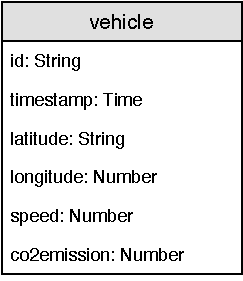
\includegraphics[width=0.2\textwidth]{db_schema}
  \caption{Database schema for storing telemetry data of vehicles in the time series database}
  \label{fig:db_schema}
\end{figure}

\subsection{CO$_2$ calculation}

An exact and efficient calculation of CO$_2$ emissions depend on many different factors, such as the model of the vehicle, year of fabrication, fuel, engine specifics and other technological features.
A good overview of the standard emission methods for vehicle emissions can be seen here \cite{potscher_co2-monitoring_2016}.
The proposed system uses a microscopic approach of simulation, in which each vehicle hast its own representation.
Individual vehicle characteristics may include factors such as vehicle type, weight, speed, acceleration, engine performance, between others.
So the level of detail is even higher at sub-microscopic models.
They can include vehicle shifting, steering, fuel consumption and so on.
Regarding of any type of model, emission can be attained into each flow model.
For this reason, the microscopic modeling is used because it helps to calculate the emission of CO$_2$ of passenger vehicles.

The method of this paper uses the following definition for the estimated emissions to approximate the generated CO$_2$ emissions as defined on \cite{behrisch_second_2015}
\begin{equation}
  \label{co2_eqn}
  P = c_{0} + c_{1}va + c_{2}va^{2}+c_{3}v+c_{4}v^{2}+c_{5}v^{3}
\end{equation}

where $P$ is the emission frequency (in miligrams per second), $c$ are the emission constants, $v$ is the vehicle's speed in $m/s$, and $a$ is the acceleration in $m/s^{2}$.
For this experiment we are going to use the constants $9449, 938.4, 0.0, -467.1, 28.26, 0.0$ respectively to be the case for gasoline driven passenger car Euro norm.
In the simulator, since we have the position, speed and acceleration of each vehicle at each given time we could potentially calculate the fuel consumption as in \cite{hofer_large_2018}.
At each received message from the vehicle, the system computes the CO$_2$ emission value and stores it along with the received data.
This will be later retrieved by a consumer.
The current implementation of emission can be extended to compute any kind of other pollutants, namely methane (CH$_4$), nitrous oxide (N$_2$O) or hydro fluorocarbons (HFC).

\begin{figure}[h]
  \centering
  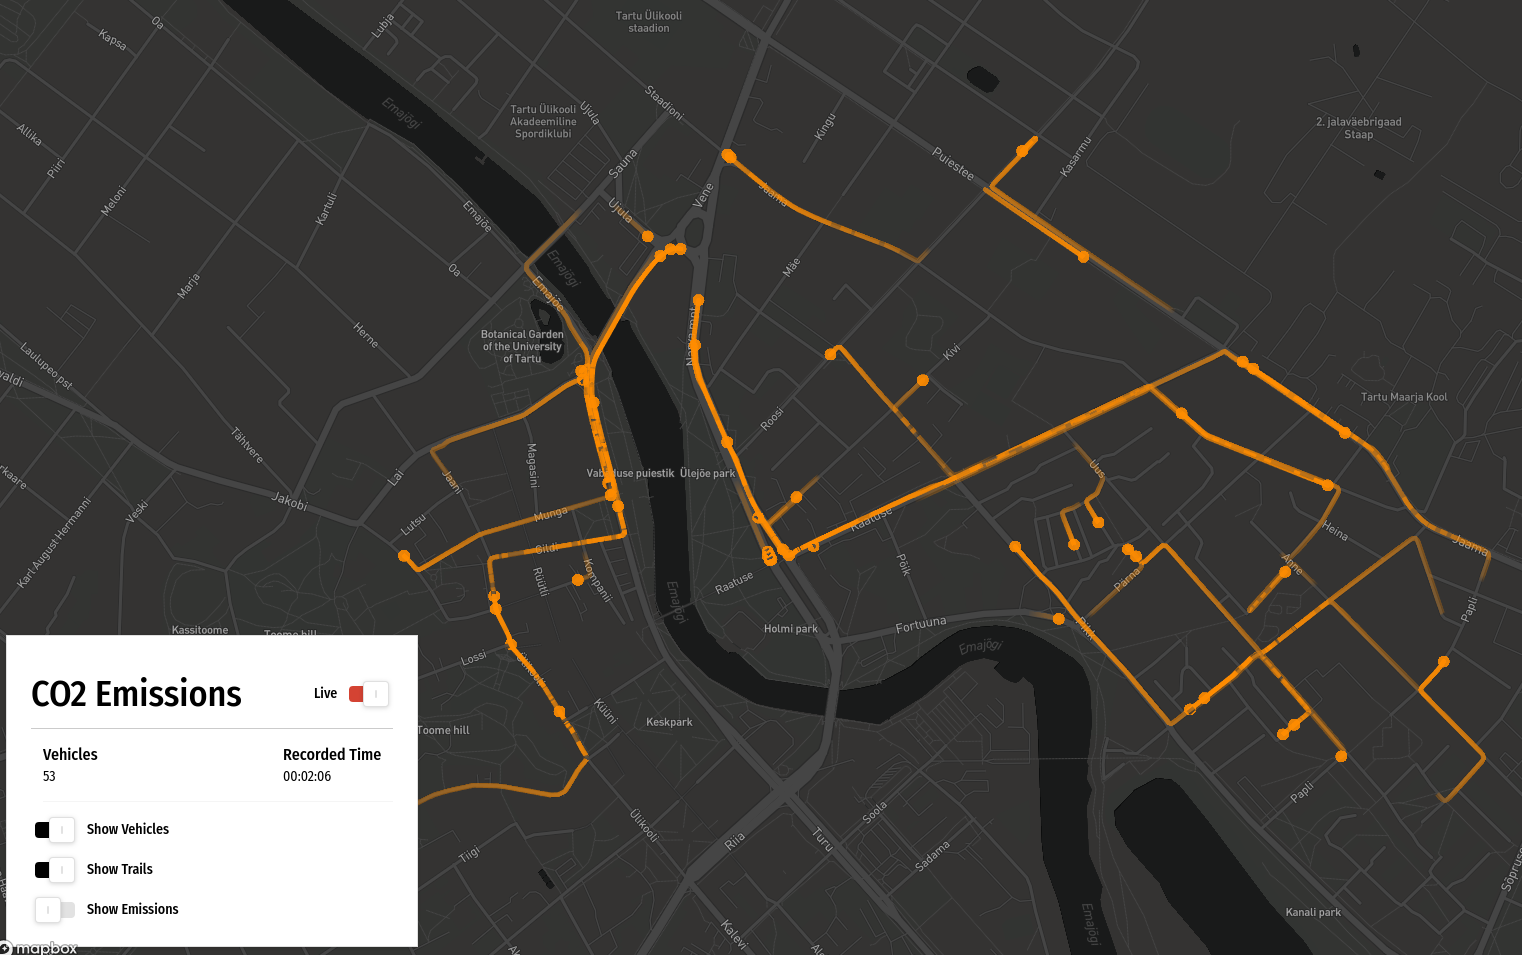
\includegraphics[width=0.45\textwidth]{app1}
  \caption{Web application in live mode showing the trace of the vehicles as they come}
  \label{fig:app1}
\end{figure}

\begin{figure}[h]
  \centering
  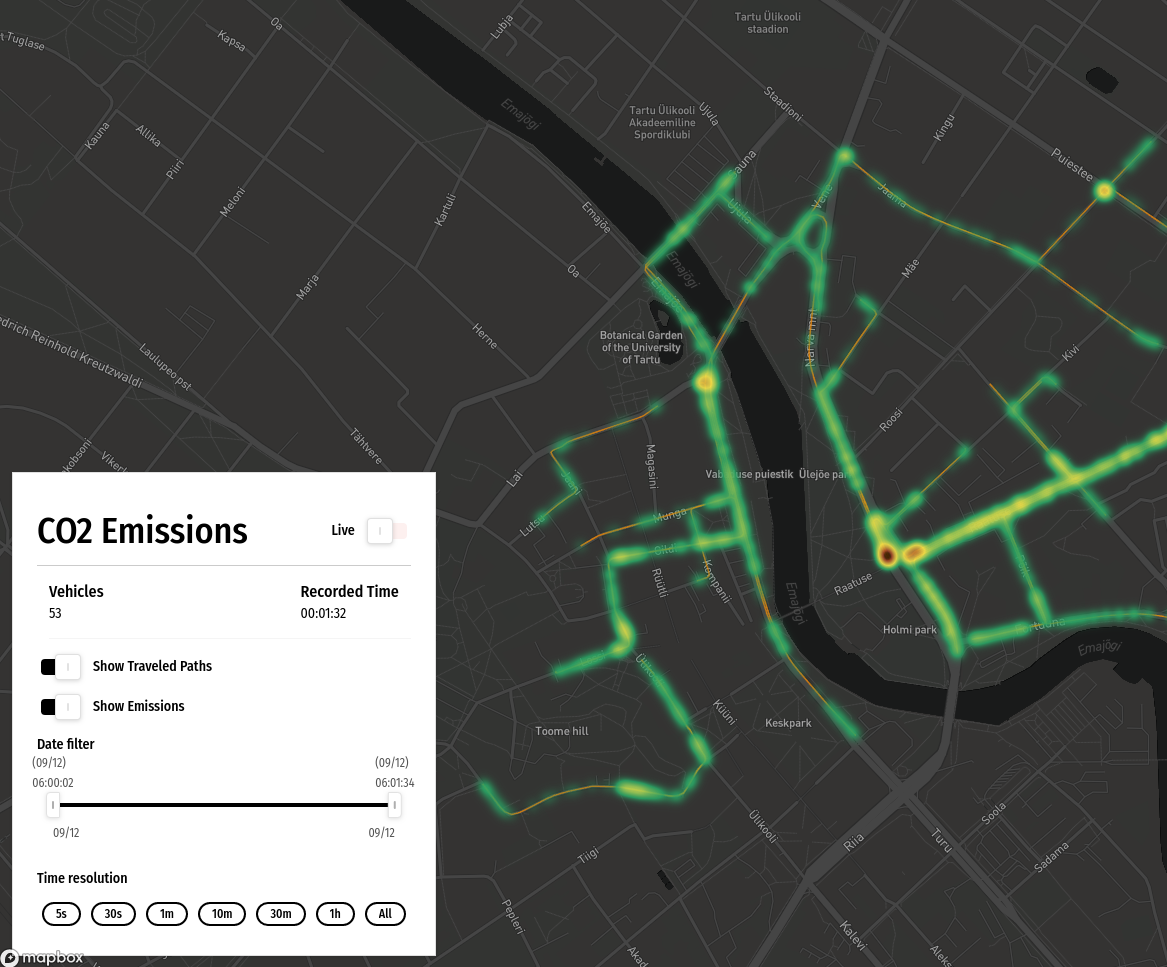
\includegraphics[width=0.45\textwidth]{app2}
  \caption{On history mode the option for filtering and showing the layers is available}
  \label{fig:app2}
\end{figure}

\subsection{Test Environment}

We need a framework to run the simulated agents into a network to make realistic trips that also could provide a test environment.
For this, we need to define a network representation of a road network.
Using SUMO to make a real-world scenario from scratch is time consuming as one needs to define and constantly tweak every single detail of the network road.
We could use the integrated SUMO tools that speed up this process, such as defining a network based on a realistic map from OpenStreetMap (OSM) \footnote{https://www.openstreetmap.org/} which contains most of the necessary information such as geographic coordinates, number of lanes, speed constrains, and so on.
Although this is a viable option, does not take into account the vehicle and trips mechanics.
This is one of the main challenges of transport simulation (if we wanted to make it close to the real world case).
As \cite{hofer_large_2018} points, data of realistic trips can be obtained directly from surveys for small-scale models, but for large scales, it is required to rely on a fine-defined estimation based on origin-destination information.
One possible fast solutions is to use the random trip script \footnote{https://sumo.dlr.de/docs/Tools/Trip.html} which defines random vehicles and trips automatically.
But still, we need to calibrate the simulation if we want to achieve a real-world traffic behavior.
As a base line scenario showed in figure \ref{fig:map1}, we use the described tool in the city of Tartu without any source modification.

\begin{figure}[h]
  \centering
  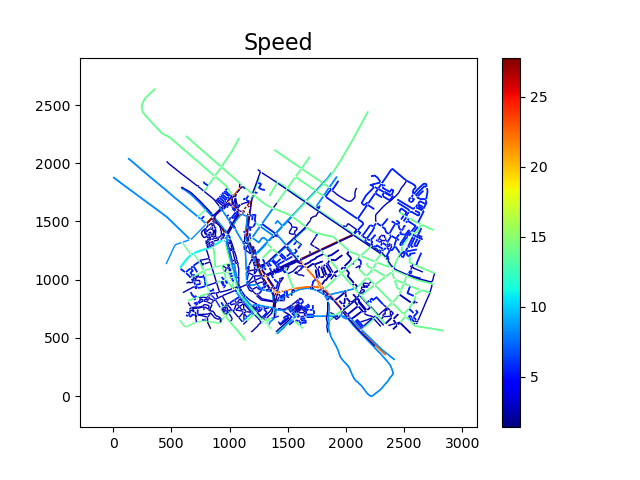
\includegraphics[width=0.45\textwidth]{map_speeds_tartu_1}
  \caption{Plot of speed on the Tartu scenario}
  \label{fig:map_speeds_tartu_1}
\end{figure}

On the other hand SUMO has several real-world and free scenarios available.
As \cite{heisig_bridging_nodate} discuss, there are four appealing scenarios to use, namely:

\begin{itemize}
  \item Bologna10
  \item The Luxembourg SUMO Traffic (LuST)
  \item The TAPASCologne, and
  \item The Monaco SUMO Traffic (MoST) \footnote{https://github.com/lcodeca/MoSTScenario}
\end{itemize}

In which the author describes the drawbacks of the first two regarding to compatibility and ease of integration.
It is then concluded that TAPASCologne and MoST is used with caution.
In our approach, the second scenario is MoST because its completeness.
The time interval for the test is between 6:00 and 10:00 am.
To help visualize the behavior of the traffic we show in \ref{fig:map_speeds_tartu_1} a plot with each depicted scenario and its respective vehicle speed results.
This was obtained with the SUMO visualization tool for plotting the network speed \footnote{https://sumo.dlr.de/docs/Tools/Visualization.html}

\begin{figure}[h]
  \centering
  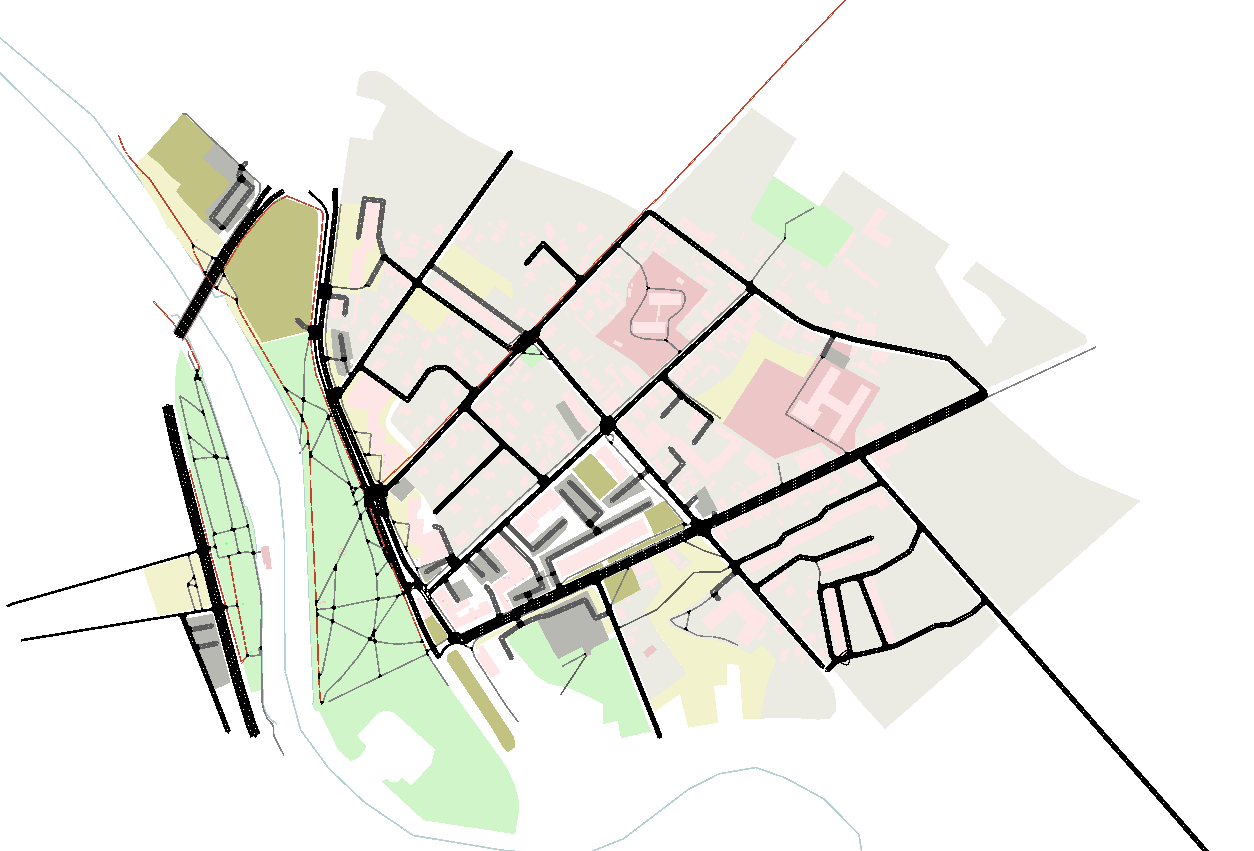
\includegraphics[width=0.45\textwidth]{map1}
  \caption{Baseline map on a small area in the city of Tartu}
  \label{fig:map1}
\end{figure}

\begin{figure}[h]
  \centering
  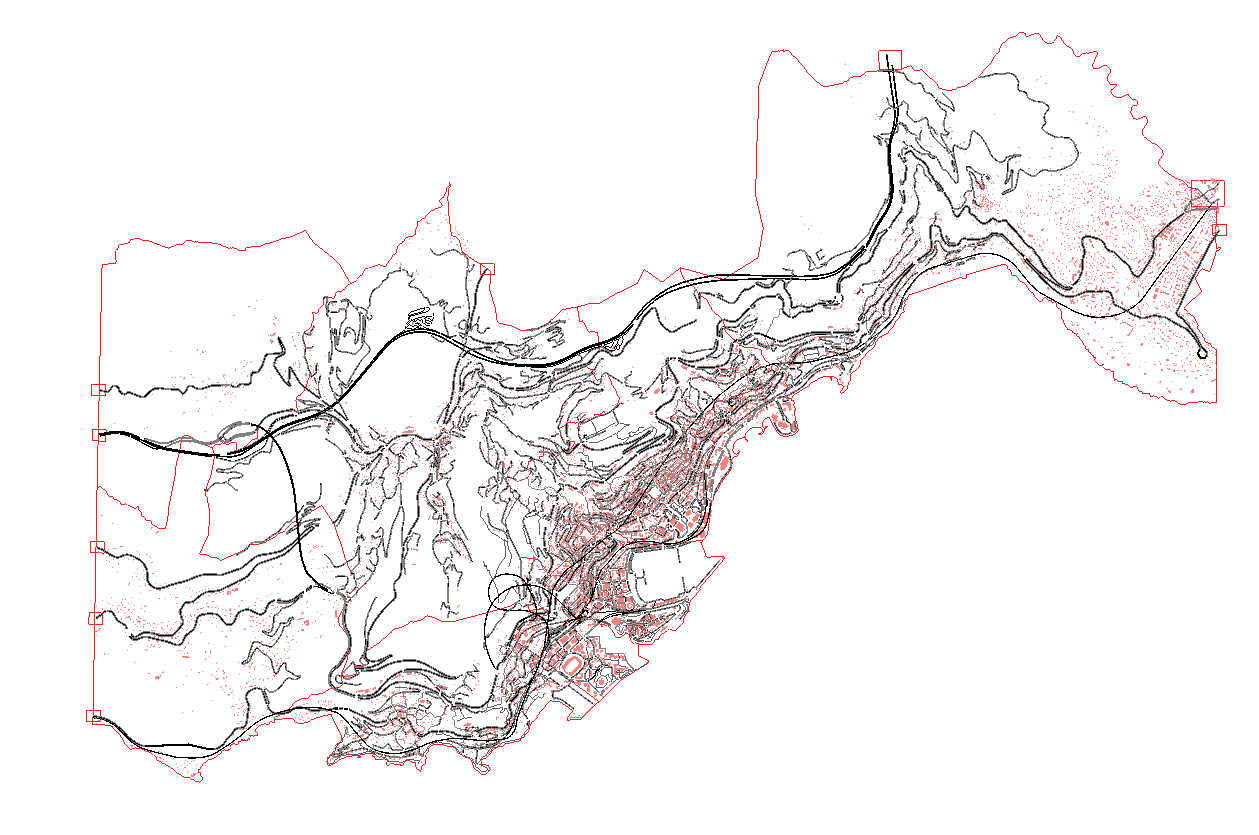
\includegraphics[width=0.45\textwidth]{map2}
  \caption{Monaco SUMO Traffic (MoST)}
  \label{fig:map2}
\end{figure}

With this described setup, the simulation in ready to run.
First the baseline scenario is executed, then it is followed by the Monaco scenario.
The simulated data gives a good insight on how this could operate in a real life.
Running the scenarios for few moments one can observe the large number of entries and hits in the database.
This became a problem when a query was needed to process to keep flexibility.
Fortunately InfluxDB allows to group and aggregate in order gain some performance.
In the figure \ref{fig:running_tartu_1} the first scenario have been running for 5 minutes.
In the figure \ref{fig:running_monaco_2} the second scenario ran for 50 minutes.
On both cases we can see the emitted CO$_2$ in the heat-map layer.
This is modified over time to fit the real-time behavior.
As we scale the view with zoom in and out the aggregation is being modified.

\begin{figure}[h]
  \centering
  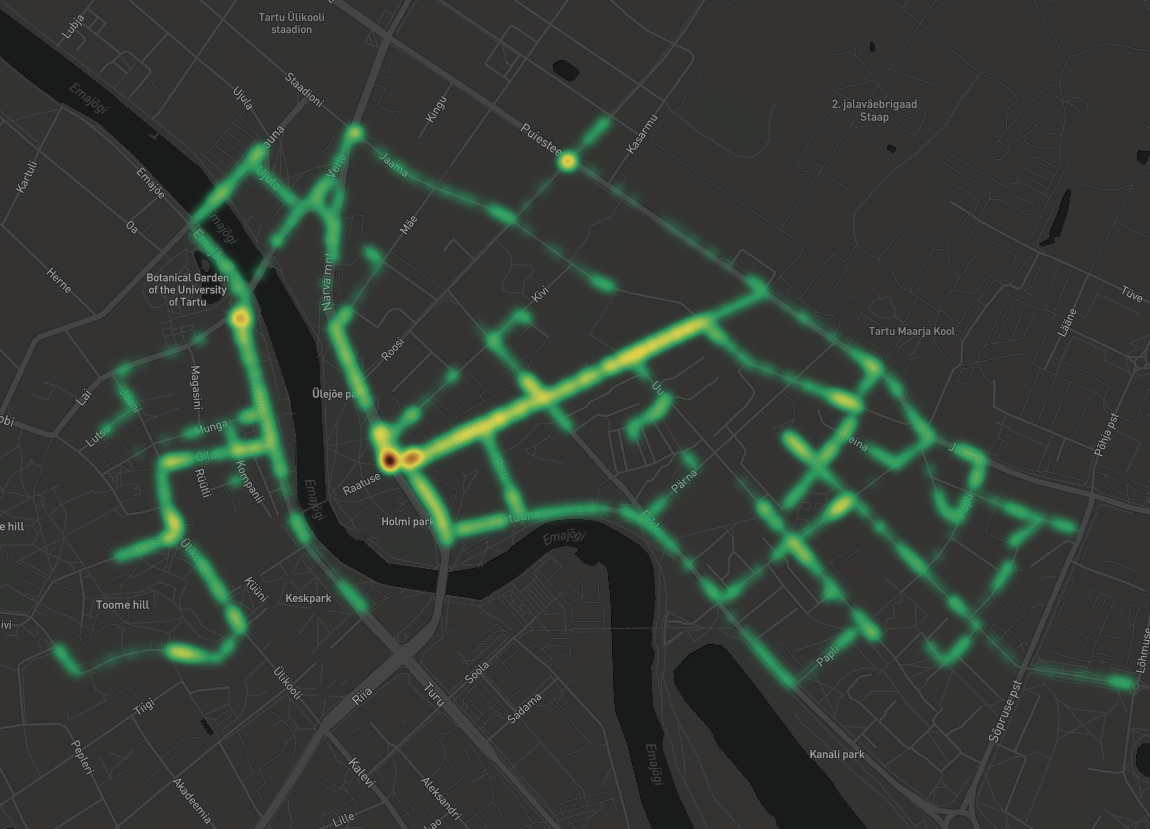
\includegraphics[width=0.45\textwidth]{running_tartu_1}
  \caption{Baseline map being executed}
  \label{fig:running_tartu_1}
\end{figure}

\begin{figure}[h]
  \centering
  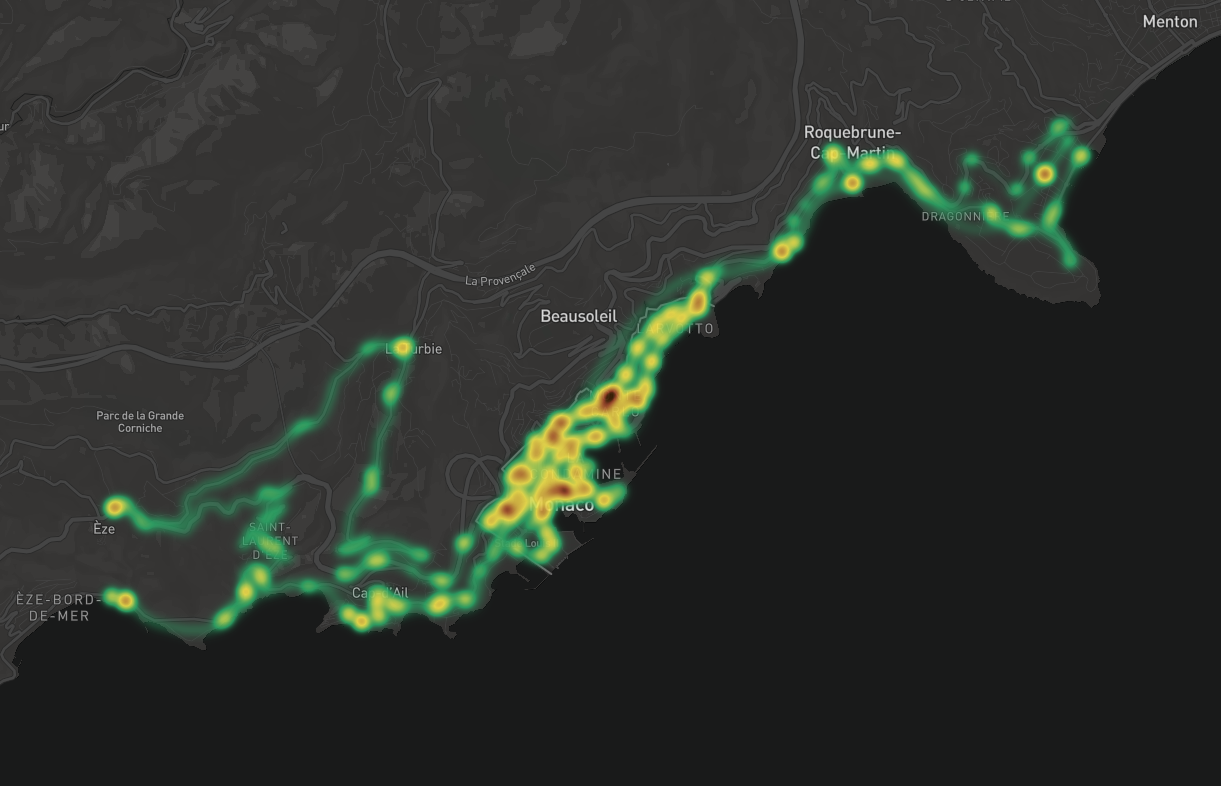
\includegraphics[width=0.45\textwidth]{running_monaco_2}
  \caption{MoST map being executed}
  \label{fig:running_monaco_2}
\end{figure}

In terms of software and hardware specifications. SUMO is running in version 1.3.1 on a local Linux machine with Intel CoreTM i7-7500U (4) CPU at 3.50GHz and 8GB RAM.
Python 3.8.0 runs under the simulation code for the TraCI integration.
Finally Nodejs version 13.3.0 runs on the server side.
There are two setups for running SUMO.
One is with graphical interface and the other without mainly with the purpose of visualizing the simultaneous vehicle behavior on both scenarios (Web app and SUMO GUI).

%%%%%%%%%%%%%%%%%%%%%%%%%%%%%%%%%%%%%%%%%%%%%%%%%%%%%%%%%%%%%%%%%%%%%%%%%%%%%%%%
\section{RESULTS}

Based on the experiment described on the previous sections, this section discusses the obtained results, the benefits of this approach, and its limitations.
Testing the first scenario revealed problems on the web application that were not addressed while initially was being developed.
This needed improvement in the code for displaying correctly the emissions over time.
Another improvement was the code for the calculation of CO$_2$, as the initial implementation of emission did not yield appealing results.
The code for the query of the database was also a thing to consider in this regard.
In parallel, debugging and running the scenarios on the SUMO graphical interface was crucial to keep the constant feedback.

In terms of CO$_2$ emission calculation, it was compared with the SUMO built-in emission model HBEFA v.2.1 \cite{behrisch_second_2015} which considers parameters of vehicle such velocity and acceleration.
In order to evaluate both under same conditions, the test was run on the same scenarios.
A quantitative estimation is used to compare both models.
According to the figure \ref{fig:tartu_emissions_plot} the SUMO model generates $5643334 mg$ of CO$_2$ emission, while the method of this paper gets $5643443 mg$.
On the second scenario showed in figure \ref{fig:monaco_emissions_plot} the SUMO model generates $8554854 mg$ of CO$_2$ emission, while the method of this paper gets $7454854 mg$.

\begin{figure}[h]
  \centering
  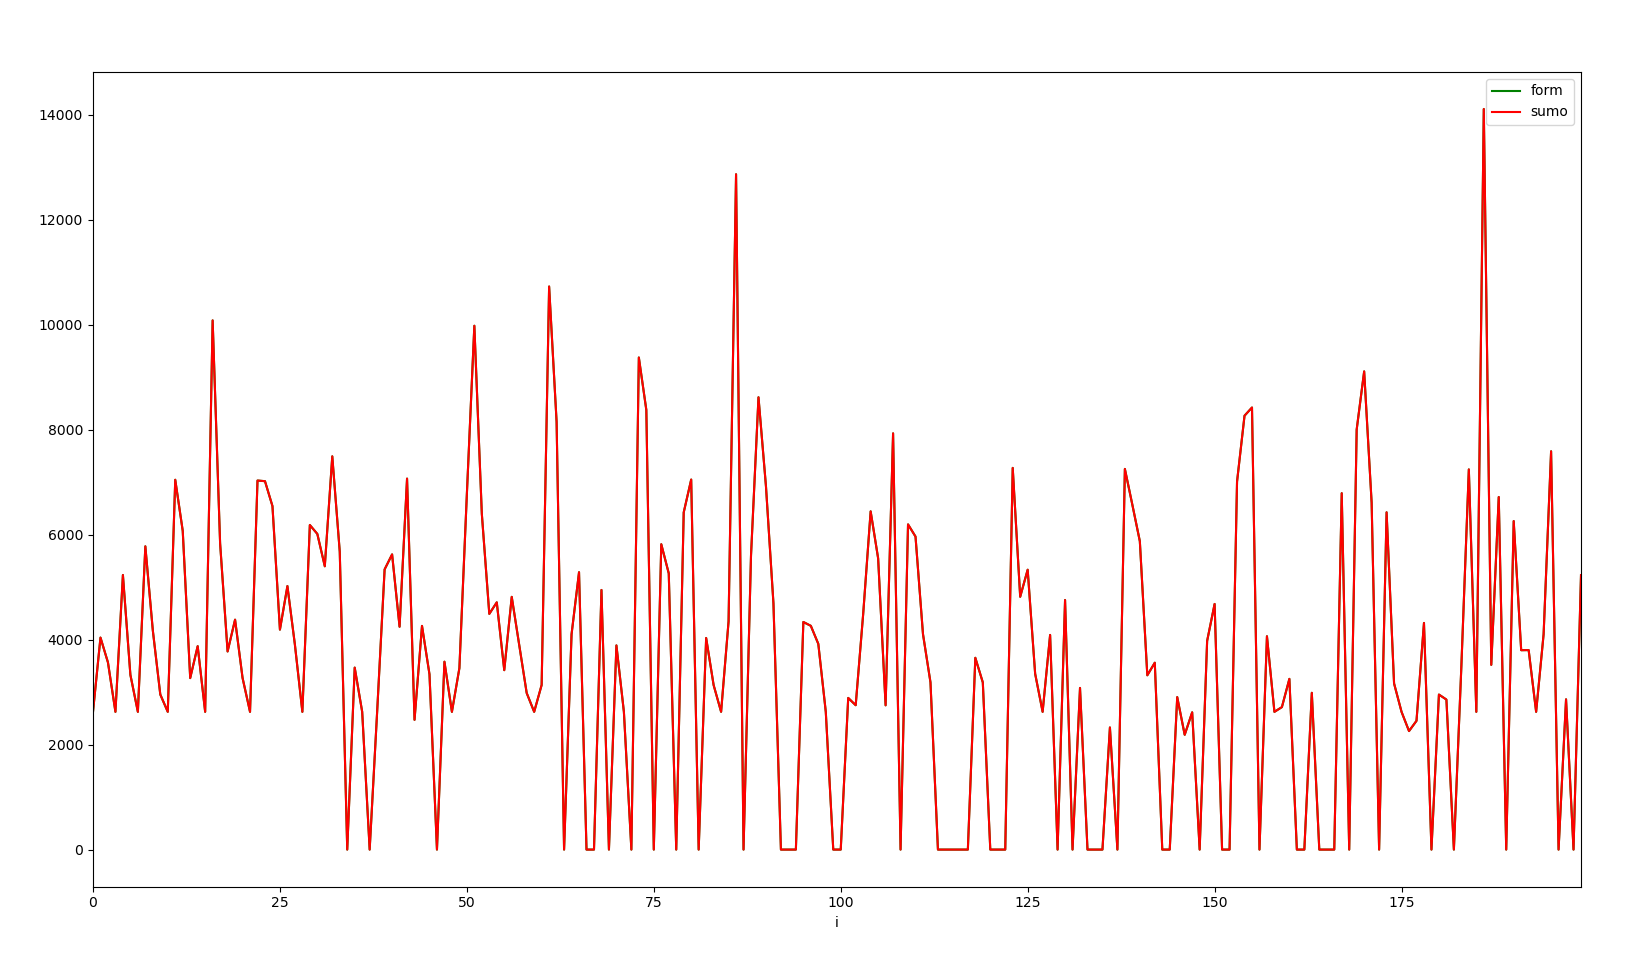
\includegraphics[width=0.45\textwidth]{tartu_emissions_plot}
  \caption{SUMO CO2 values vs own implementation shows a mean error or 1\% on baseline scenario}
  \label{fig:tartu_emissions_plot}
\end{figure}

\begin{figure}[h]
  \centering
  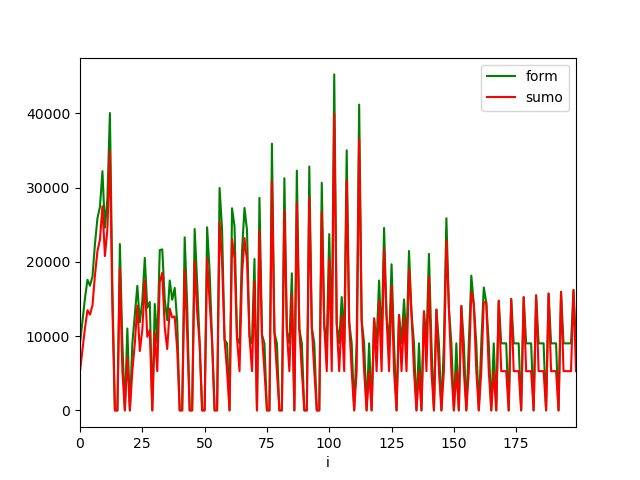
\includegraphics[width=0.45\textwidth]{monaco_emissions_plot}
  \caption{SUMO CO2 values vs own implementation shows a mean error or 15\% on MoST scenario}
  \label{fig:monaco_emissions_plot}
\end{figure}

Achieving the real-time support for showing the emission was the most challenging part of this project since for complex scenarios the system required more computational resources.
For evaluating the architecture of the system, the emulation of vehicles with SUMO was the key.
It was even relatively easy to run concurrent test cases on a separate environment.

It is always discussed in the ITS traffic literature that electric cars emit less emission than old traditional cars.
This is a consideration and improvement that could be added to a new version of the system.
We could also add more pollutants based on vehicle and environment parameters.
Also a point to consider is the realistic representation of a city because if we were to run on it we could make better decisions in terms of ITS policies.
Note, that this system was only concerned with CO$_2$ emissions and its applicability to the existing devices (i.e. mobile phones) into a visualization tool taking into consideration its reliability through a distributed approach.
The ultimate goal of this kind of simulations is to make effect on improving the environment quality.

%%%%%%%%%%%%%%%%%%%%%%%%%%%%%%%%%%%%%%%%%%%%%%%%%%%%%%%%%%%%%%%%%%%%%%%%%%%%%%%%
\section{CONCLUSIONS}

With an increasing number of connected vehicles on the road, traffic congestion has become a daily problem affecting several aspects of modern society.
One of the problems of traffic that concerns more to the environment is the pollution through the CO$_2$ emission.
We also have noticed that nowadays we have an scenario of vehicle drivers somehow connected to a cloud service, this can be leveraged to use them in order to get estimation of CO$_2$ emission into the current state of traffic.
A system was proposed to fulfill this requirement.
It was discussed the necessity for building a solution and why it should be developed in a distributed way.
Hopefully the visualization tool provides an insight in the decision making of ITS policies.

\addtolength{\textheight}{-12cm}

%%%%%%%%%%%%%%%%%%%%%%%%%%%%%%%%%%%%%%%%%%%%%%%%%%%%%%%%%%%%%%%%%%%%%%%%%%%%%%%%

\bibliography{references}
\bibliographystyle{ieeetr}

\end{document}